\documentclass[10pt]{ocsmnar}



% Adjust this to the language used.
\usepackage[ngerman]{babel}
\usepackage{hyperref}
\usepackage{amsmath}
\seminar{Praxismodul}
\semester{Sommersemester 2020}

\begin{document}


\title{Implementierung und Evaluation von Mixing-Modell-Alternativen für XCS}


\author{Markus Weis}

\maketitle




\section{Einleitung}
In modernen Michigan-Style Learning Classifier Systemen (LCS) wird üblicherweise aus einzelnen Classifier Vorhersagen eine Gesamtvorhersage berechnet. In XCS wird die Prediction über eine Fitness gewichtete Summe der einzelnen Predictions berechnet. Diese Fitness ist ein heuristisch Parameter, der inkrementell berechnet wird. Wilson schreibt, dass es wohl verschieden Möglichkeiten gibt die Gesamtvorhersage zu berechnen, behält aber dieses Modell ohne weitere Ausführung in seinen späteren Arbeiten bei \cite{Wilson95}. 
Drugowitsch setzt in seinem Buch "Design and Analysis of Learning Classifier Systems - A Probabilistic Approach" \cite{book} dort an. Er beschreibt verschiedene Mixing Modelle und wertet diese empirisch aus. 
Eines dieser Modelle wird in der vorliegenden Arbeit beschrieben und eine Implementierung versucht: Inverse Variance Mixing. Aus den heuristisch Modellen schnitt dieses stets am besten ab, während die Laufzeit der  analytischen Lösung nicht angemessen ist. Das Modell wird im Open-Source Projekt scikit-XCS \cite{repo}, einer scikit-learn Erweiterung für XCS, implementiert. Und anschließend ausgewertet, ob es sich um eine sinnvolle Mixing-Alternative handelt.

\section{Inverse Variance Mixing}
Die Definition des Inverse Variance Mixing ist \cite{book} entnommen. 

$$ \tau_{k}^{-1} = (c_{k} - D^{X}) \sum_{n}^{N} m_{k}(x_{n}) (\hat{w}_{k}^T x_{n} - y_{n})^{2}$$

Dabei ist $\tau_{k}^{-1}$ die Varianz und folglich $\tau_{k}$ die inverse Invarianz. $C_{k}$ ist der Matchcount des Classifiers k, $D^{X}$ ist die Dimension des Input Raums. $m_{k}(x)$ ist eine Matching-Funktion für die gilt: $m_{k}(x) = 1$, falls die Bedingung des Classifiers k auf x passt und $m_{k}(x) = 0$ sonst. 
Der hintere Term stellt das quadratische Fehlermaß der Regression dar. Dieser muss hier angepasst  werden, da Klassifikation implementiert werden soll.

Die erste Implementierung lautet wie folgt: 

$$ \tau_{k}^{-1} = (c_{k} - D^{X}) \sum_{n}^{N} m_{k}(x_{n})f_{k}(x_{n}) $$

Wobei $f_{k}(x)$ den Klassifikationsfehler darstellen soll: $f_{k}(x) = 0$, falls Classifier k die richtige Klasse für Input x hat und $f_{k}(x) = 1$, sonst. 

Später wurde statt der Klasse der Fehler der Prediction als Fehlermaß verwendet:

$$ \tau_{k}^{-1} = (c_{k} - D^{X}) \sum_{n}^{N} m_{k}(x_{n}) |p_{k} - P_{k}(x)|  $$

$p_{k}$ ist die Prediction des Classifiers k, $P_{k}(x)$ ist der Reward, der ausgeschüttet wird, wenn Classifier k auf Input x seine Klasse vorhersagt. 
Anstelle des Betrags wurde auch versucht den Fehler zu quadrieren, dies hatte aber keine relevanten Auswirkungen.

Schließlich wird die inverse Varianz nicht direkt benutzt, sondern  der sog. Gating Parameter $g_{k}$ über das aktuelle Matchset berechnet: 
$$ g_k(x) = \frac{m_k(x)\tau_k}{m_i(x)\sum_i^K \tau_i}$$

Dadurch wird sichergestellt, dass die Summe aller Gating Parameter für jeden Input 1 ergibt. 




\section{Probleme}
Im Buch wurde Inverse Variance Mixing nie im XCS-Context benutzt. Stattdessen wurde sie im allgemeineren Context von LCS definiert. LCS Classifier im Buch wurden durch Batch Learning trainiert und nicht iterativ, wie es bei XCS der Fall ist. 
Ein erster Ansatz der Implementierung hier war einfach die Fitness der einzelnen Classifier durch die inverse Variance zu ersetzten. 
Daraus ergaben sich aber 2 Probleme: 

1. Da man für alle Classifier, die für die aktuelle Prediction verantwortlich sind, die Fitness updatet, müsste man für alle diese die inverse variance neu berechnen. Dazu wird aber für jeden Classifier das komplette Trainingsset durchlaufen. Dies führt zu einer nicht akzeptablen Laufzeit. Hier müsste wie im restlichen XCS ein iterativer Ansatz verfolgt werden. Dies wurde hier nicht gemacht, da man sich dadurch noch weiter von der ursprünglichen Idee entfernt und weiter Hyperparameter eingefügt werden müssten. 
Stattdessen wurde die Laufzeit erstmal in Kauf genommen und geschaut, ob auf diese Weise gute Ergebnisse auftreten.  

2. Das Erzeugen neuer Classifier benutzt die Fitness als Auswahlkriterium. Allerdings ist die Inverse Variance zu Beginn des Training Vorgangs noch nicht als sinnvoll zu betrachten. Beispielsweise wird ein Classifier, der auf einen Input perfekt passt stets bevorzugt, egal ob es Allgemeinere gibt, die ähnlich gut und eventuell allgemeiner sind.  

Wir sind schließlich zu dem Schluss gekommen, die Fitness des ursprünglichen XCS Systems in Ruhe zu lassen und die Inverse Variance nur für das Mixing zu benutzten. Das Problem mit der Laufzeit bleibt aber bestehen, da die Prediction bei nicht Explorationsiterationen für die Auswahl der Action berechnet werden muss. Schließlich wurden 2 Alternativen implementiert. Die eine macht die Prediction während des Trainings bereits mit der inversen Invarianz und zeigt deshalb eine sehr schlecht Laufzeit auf. Bei der anderen wird die neue Mixing Art nur bei Predictions benutzt, die nicht während des Trainings auftreten, also nur im fertigen Model. Das hat den Vorteil, dass die inverse Varianz für alle Classifier am Ende des Trainingsprozesses berechnet werden kann und für die einzelnen Prediction nur der Gating Parameter aktualisiert werden muss.  
 


Wie bereits beschrieben handelt es sich bei der eigentlichen Definition um Regression. Bei Regression ist es unwahrscheinlich bzw. unmöglich, je nach Modell, auf einen perfekten Classifier zu treffen. Das Problem bei einem perfekten Classifier ist, dass der hintere Teil der Formel, also das Fehlermaß, Null ergibt. Das wird zum Problem, wenn man zur Berechnung der Inversen Varianz den Umkehrbruch bildet. Im Buch ist das nicht weiter definiert. In dieser Implementierung habe ich in diesem Fall Unendlich (numpy.inf) eingesetzt. Dadurch bekommt man schließlich im Mixing Probleme. Zwar bekommt man bei einem Mixing-Parameter mit  $\tau_{k} =   \infty$ bei allen anderen Classifiern, die nicht Unendlich als inverse Varianz haben, 0 raus, allerdings ist $\frac{\infty}{\infty}$ bzw. $\frac{numpy.inf}{numpy.inf}$ nicht definiert, was für alle Classifier mit $\tau_{k}^{-1} = \infty$ geschieht:

$$ g_k(x) = \frac{m_k(x)\tau_k}{m_i(x)\sum_i^K \tau_i} = \frac{\infty}{\infty} $$

Stattdessen wird $g_{k}$ im Falle eines Classifiers k im Matchset mit $\gamma_{k} = \infty$ wie folgt berechnet: $g_{k} = \frac{1}{c_{inf}} $ für alle Classifier k mit $\gamma_{k} = \infty$ und $g_{k} = 0$ für alle anderen Classifier. $c_{inf}$ ist die Anzahl der Classifier mit $\gamma_{k} = \infty$.

Ein weiteres Problem ergab sich im Fall, dass der Matchcount $c_k$ für einige Classifier geringer als die Dimension des Inputs war, sodass sich für die Varianz und die negative Varianz ein negativer Wert ergibt. Im Buch ist nicht beschrieben, wie in diesem Fall mit den Classifiern umgegangen werden soll. Im meiner Implementierung werden diese Classifier einfach ignoriert. 



\section{Ergebnisse}
Die Implementierung wurde auf Multiplexern verschiedener Größe evaluiert: 6 Bit, 11 Bit und 20 Bit. Die Trainingsdauer und die Hyperparameter orientieren sich an \cite{iqbal13}. Dort ist zu entnehmen, wie viele Iterationen XCS braucht, um die verschieden großen Multiplexer perfekt zu lernen. Letztendlich wäre jedes der hier zu evaluierenden Implementierungen bei den Problemen zu einer perfekte Accuracy gekommen, wenn man nur lange genug trainiert. Es wäre wohl sinnvoll die Implementierungen auch auf Problemen zu testen, bei denen XCS keine perfekte Lösung finden kann. Dies wird hier allerdings nicht gemacht. 
Es wird für 4000, 10000, 40000 Iterationen für den 6-Bit, 11-Bit und 20-Bit Multiplexer trainiert. 
Die durchschnittliche Accuracy der Cross\--Vali\-dation der verschiedenen Implementierungen ist der Tabelle \ref{accuracy-tabelle}
 zu entnehmen. Dabei wird jeweils eine 10x5 Cross-Va\-li\-da\-tion durchgeführt. Es sei hier nochmal erwähnt, dass das kontinuierliche Update der inversen Varianz zu sehr langsamer Laufzeit führt und deshalb die Ergebnisse nicht auf größeren Datensätzen ausgewertet werden können. 
Es wird neben den beiden bereits erwähnten Implementierungen der inversen Varianz noch eine Gleichgewichtung der Classifier vorgenommen, um den Effekt des Mixings vergleichen zu können (evenly-distributed).  

\begin{table}
    
\begin{center}\label{accuracy-tabelle}
\begin{tabular}{|c|c|c|c|}
    \hline
    & 6 Bit & 11 Bit & 20 Bit \\
    \hline
    normal & 0,98 (+/- 0,03) & 0,98 (+/- 0,02) & 0,89 (+/- 0,05) \\
    \hline
    evenly-distributed & 0,88 (+/- 0,06) & 0,92 (+/- 0,04) & 0,84 (+/- 0,05) \\
    \hline
    only-mixing & 0,87 (+/- 0,06) & 0,90 (+/- 0,04) & 0,84 (+/- 0,05) \\
    \hline
    continuous-update & 0,93 (+/- 0,04) & 0,93 (+/- 0,03) & 0,85 (+/- 0,05) \\
    \hline
\end{tabular}
\end{center}
\caption{Durchschnittliche Accuracy der verschiedenen Implementierung mit Standartabweichung in Klammern. }\label{accuracy-tabelle}
\end{table}

Es ist hier bereits zu erkennen, dass die Ergebnisse des inverse Variance Mixing schlechter sind als die des normalen XCS-Mixing. 
Genauere Auswertungen der verschiedenen Problem-Größen sind hier aufgeführt. 

\subsection{6 Bit Multiplexer}
Die Boxplots zu den Accuracy Werten aus Tabelle \ref{accuracy-tabelle} sind in Abbildung \ref{boxplot-6-bit} zu sehen. Das normale XCS schneidet am besten ab. Evenly-distributed ist zwar auf einem ähnlichem Niveau, wie die beiden Inverse Variance Arten, allerdings hat es einige negative Ausreißer. 


\begin{figure}
    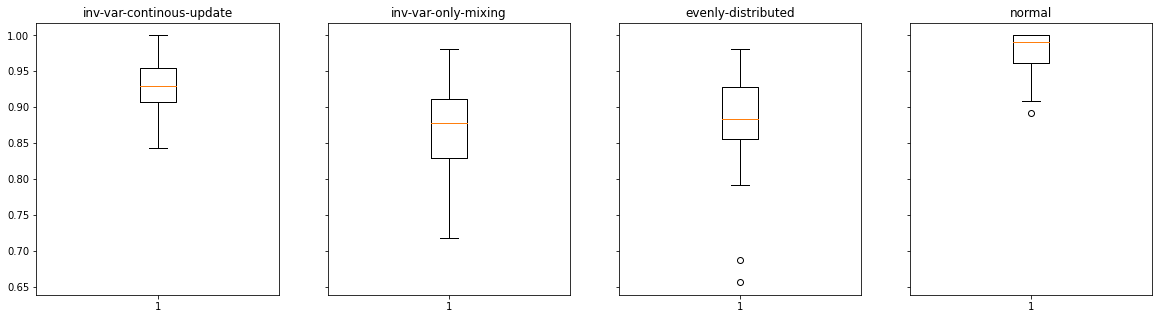
\includegraphics[width=\linewidth]{img/boxplot_6Bitpng.png}
    \caption{Accuracy Werte des 6 Bit Multiplexers}
    \Description[short]{long}\label{boxplot-6-bit}
\end{figure}

Schließlich wurde noch ein TTest durchgeführt, um zu überprüfen, ob die Unterschiede der Algorithmen statische Signifikanz aufweisen. Hierfür wurde die Funktion $paired\_\-ttest\-\_5x2cv()$ der MLxtend Library von Sebastian Raschka verwendet. Es wurde ein Signifikanzwert von $\alpha = 0,05$ verwendet. Das bedeutet die Unterschiede zwischen den Implementierungen sind signifikant, falls das Ergebnis der des $paired\_\-ttest\-\_5x2cv()$ einen Wert unter 0,05 liefert. Diese Einträge sind gelb hinterlegt. Die Ergebnisse sind Abbildung \ref{ttest-6-bit} zu entnehmen. 

\begin{figure}
    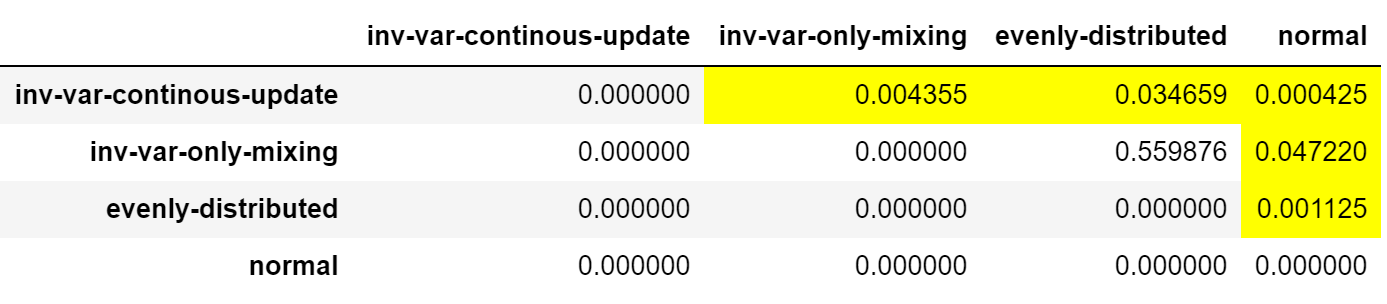
\includegraphics[width=\linewidth]{img/ttest_6_bit.png}
    \caption{5x2 Cross-validation paired ttest auf dem 6 Bit Multiplexer}\label{ttest-6-bit}
    \Description[short]{long}
\end{figure}

Der TTest erkennt unterschiede zwischen allen Verteilungen, außer zwischen evenly-distributed und inv-var-only-mixing. Dies spricht gegen die Verwendung der inv-var-only-mixing Implementierung.

\subsection{11 Bit Multiplexer}

Die Boxplots sind in Abbildung \ref{boxplot-11-bit} zu sehen. Wieder schneidet das normale XCS am besten ab. Die Accuracy von \textit{normal} ist mit 0,98 genauso gut wie beim 6 Bit Multiplexer. Allerdings sind die anderen Implementierung mindestes genauso gut, wie ihre entsprechende Ausführung auf dem 6 Bit Multiplexer.  Das liegt bei den Inverse-Variance-Mixing-Alternativen wahrscheinlich an der größeren Menge an Trainingsbeispielen, die unabhängig von der Anzahl der Trainingsiterationen durchlaufen werden. 

Der TTest erkennt hier Unterschiede zwischen allen Verteilungen (siehe Abb. \ref{ttest-11-bit})

\begin{figure}[h]
    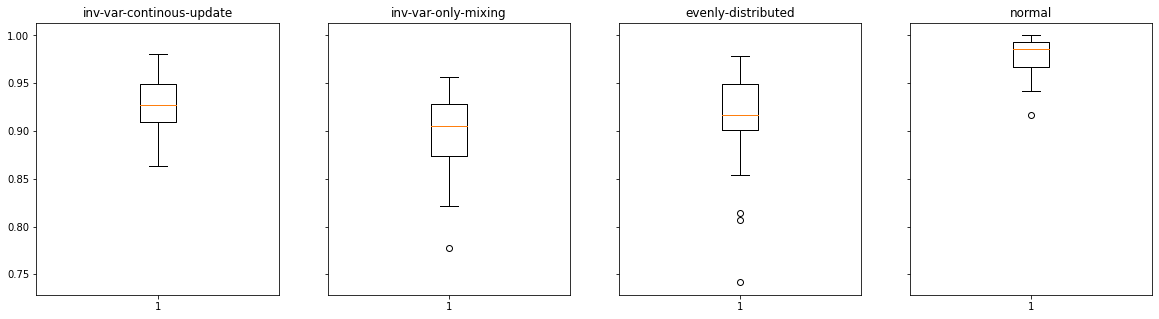
\includegraphics[width=\linewidth]{img/boxplot_11_bit.png}
    \caption{Accuracy Werte des 11 Bit Multiplexers}\label{boxplot-11-bit}
    \Description[short]{long}\label{boxplot-11-bit}
\end{figure}

\begin{figure}[h]
    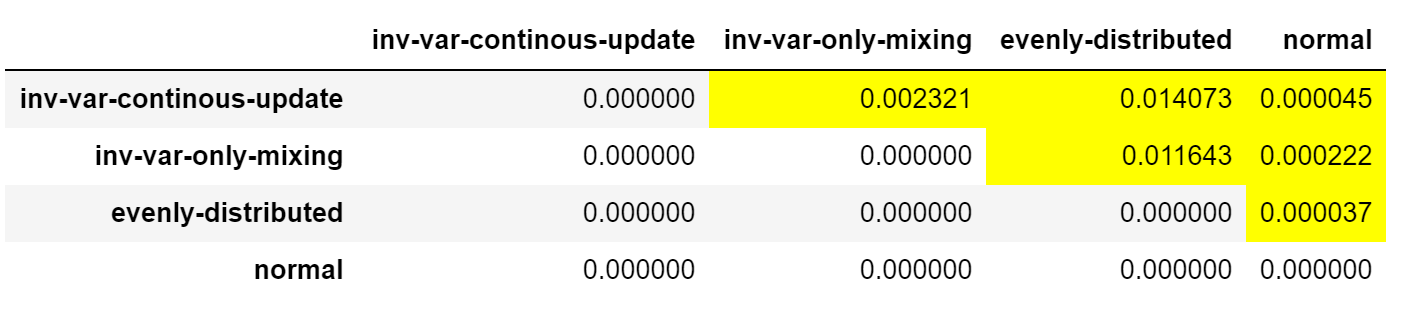
\includegraphics[width=\linewidth]{img/ttest_11_bit.png}
    \caption{5x2 Cross-validation paired ttest auf dem 11 Bit Multiplexer}\label{ttest-11-bit}
    \Description[short]{long}
\end{figure}

\subsection{20 Bit Multiplexer}

In Abbildung \ref{boxplot-20-bit} ist zu sehen, dass die Accuracy aller Implementierungen nicht das Niveau der kleineren Multiplexern erreicht. Bei längerem Training hätte sich die Performance wohl noch verbessert, allerdings war beim 20 Bit Multiplexer schon die Grenze erreicht, bei der das kontinuierliche Update noch in vernünftiger Laufzeit ausführen ließ. Das liegt vor allem an der großen Anzahl der Trainingsbeispiele (2000), die bei jeder Iteration für jeden Classifier komplett durchlaufen werden muss. 
Wieder schneidet \textit{normal} am besten ab: 0.89. Die anderen Implementierungen liegen mit 0,84 - 0,85 knapp dahinter. Der Vorsprung von \textit{normal} ist nicht so groß wie bei den 6 und 11 Bit Multiplexern.
\textit{evenly-distributed} ist wieder fast so gut, wie \textit{continuous-update} und \textit{only-mixing}.  
Der TTest bestätigt diese Eindrücke teilweise: Zwischen \textit{only-mixing} und \textit{continuous-update} besteht kein signifikanter Unterschied. Er besagt allerdings auch, dass \textit{normal} und \textit{continuous-update} keine unterschiedlichen Verteilungen besitzen. Da die Laufzeit von \textit{continuous-update} aber wie bereits beschrieben derart schlecht ist, ist \textit{normal} weit besser. 


\begin{figure}[h]
    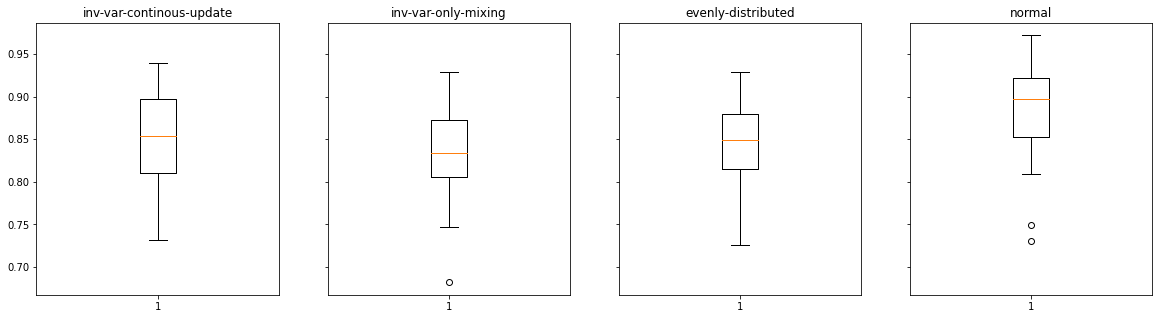
\includegraphics[width=\linewidth]{img/boxplot_20_bit.png}
    \caption{Accuracy Werte des 20 Bit Multiplexers}
    \Description[short]{long}\label{boxplot-20-bit}
\end{figure}


\begin{figure}[h]
    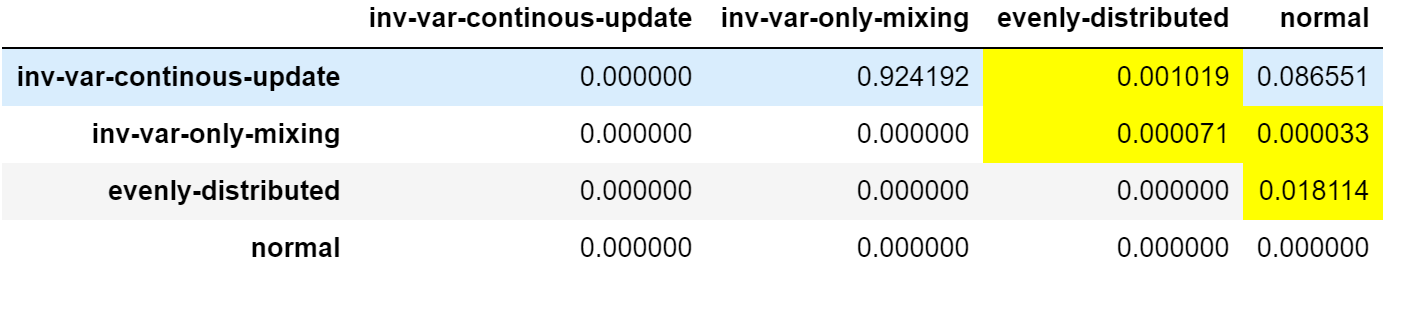
\includegraphics[width=\linewidth]{img/ttest_20_bit.png}
    \caption{5x2 Cross-validation paired ttest auf dem 20 Bit Multiplexer}\label{ttest-20-bit}
    \Description[short]{long}
\end{figure}


\section{Fazit}
Die hier beschrieben Ergebnisse zeigen, dass das Inverse Variance Mixing, wie es hier implementiert ist, sicher nicht als sinnvolle Alternative zum gewöhnlichen XCS-Mixing benutzt werden kann. In dieser Implementierung wurde allerdings notwendigerweise stark von der eigentlichen vorgeschlagenen Heuristik abgewichen. Welche der Abweichungen zu den schlechten Resultaten führt ist schwer zu sagen. 
Es handelte sich hierbei eher um einen praktischen Versuch und die formale Korrektheit wurde dabei vernachlässigt. Dies war aufgrund der Komplexität des Themas und der beschränkten Zeit notwendig. Es kann also sein, dass es durchaus sinnvolle Implementierung von Inverse Variance Mixing in XCS gibt, v.a. da hier nur Klassifikation betrachtet wurde. 
Auffällig ist, dass das Mixing mit gleicher Verteilung der Classifier relativ gut abschneidet. Dies deutet darauf hin, dass das XCS Mixing nicht optimal ist. Weiter Mixing Modelle sollten daher ausprobiert werden.  



\bibliographystyle{ACM-Reference-Format}
\bibliography{References}


\end{document}
